\section{Descrição de Hardware}
O objetivo principal do hardware é fornecer os meios eletrônicos e físicos para coletar os dados necessários para o controle de trajetória do foguete d'água e para automatizar o processo de lançamento. Isso envolve a integração de sensores para medir parâmetros como pressão, ângulo, altitude, velocidade e aceleração. O hardware é projetado para trabalhar em conjunto com o software, onde os dados coletados pelos sensores são processados e utilizados para analisar a trajetória do foguete. A escolha dos componentes de hardware é feita para garantir que eles atendam aos requisitos de desempenho do software, como a precisão das medições e o armazenamento dos dados.

Para cumprir o objetivo de coletar dados de voo e controlar o sistema de lançamento, o hardware é implementado utilizando o microcontrolador ESP32 como o componente central de processamento. O desenvolvimento do código para o ESP32 será realizado na Arduino IDE (Integrated Development Environment), uma plataforma de desenvolvimento integrada que simplifica significativamente o processo de escrita, compilação, upload e depuração do código para microcontroladores. A escolha da Arduino IDE se deve à sua facilidade de uso, vasta comunidade de suporte e disponibilidade de bibliotecas, o que acelera o desenvolvimento e reduz a complexidade do projeto. A linguagem de programação utilizada será a "C", devido à sua eficiência, controle de baixo nível e adequação para sistemas embarcados onde o desempenho e o uso eficiente de recursos são críticos.

O microcontrolador ESP32 é responsável por orquestrar a coleta, o pré-processamento e o armazenamento dos dados provenientes dos sensores. Para facilitar a interação com os diversos periféricos e garantir a modularidade e a reutilização do código, serão utilizadas bibliotecas específicas:

Para a comunicação com o módulo de cartão SD (MH-SD Card Module), será utilizada a biblioteca SD.h, que fornece um conjunto robusto de funções para leitura e escrita de dados em cartões SD no formato FAT32. Essa biblioteca permite a criação, abertura, leitura, escrita e fechamento de arquivos, bem como a manipulação de diretórios, garantindo a persistência dos dados de voo para análise posterior.

Para a leitura dos dados do sensor MPU-6050, será utilizada a biblioteca Adafruit MPU6050 (ou similar), que abstrai a complexidade da comunicação I2C com o sensor e fornece funções para a obtenção de dados de aceleração e velocidade angular em três eixos. Essa biblioteca simplifica a calibração do sensor e a conversão dos dados brutos em unidades físicas, facilitando o desenvolvimento do firmware.

O controle do motor DC através do módulo Ponte H L298N será realizado diretamente pelos pinos GPIO da ESP32. A velocidade do motor será ajustada via modulação por largura de pulso (PWM) no pino Enable (EN) da Ponte H, enquanto a direção de rotação será definida através de sinais HIGH/LOW enviados aos pinos de entrada (IN1 e IN2) da Ponte H, permitindo o acionamento preciso da trava de lançamento.

O sensor MPU-6050, um componente essencial para a medição da orientação e do movimento do foguete, é instalado estrategicamente no foguete para capturar com precisão a aceleração e a velocidade angular durante o voo. Os dados coletados por este sensor são cruciais para a reconstrução da trajetória do foguete e para a análise do seu desempenho. Especificamente, o MPU-6050 fornece dados de aceleração linear nos três eixos cartesianos $(x,y \text{ e } z)$, permitindo determinar as forças que atuam sobre o foguete em cada direção, através da aplicação da segunda lei de Newton. A velocidade angular, também medida nos três eixos, é fundamental para compreender a rotação e a estabilidade do foguete durante o voo. A integração temporal dos dados de aceleração, combinada com a orientação obtida da velocidade angular, possibilita o cálculo do deslocamento do foguete ao longo do tempo, fornecendo informações detalhadas sobre a sua posição e trajetória no espaço.

Simultaneamente, um módulo de leitura de cartão SD (MH-SD Card Module) é integrado ao sistema para fornecer um meio de armazenamento local e não volátil para os dados de voo, atuando como um backup e garantindo que nenhum dado crítico se perca, mesmo em caso de falhas.

A arquitetura do firmware seguirá os princípios de sistemas de tempo real, priorizando a eficiência e o determinismo na execução das tarefas. O firmware será estruturado em um loop principal contínuo e determinístico, responsável pela execução cíclica das seguintes tarefas:
\begin{itemize}
    \item Leitura dos dados dos sensores: Os dados dos sensores, incluindo o MPU-6050, são amostrados periodicamente com uma frequência predefinida para garantir a captura adequada da dinâmica do voo.
    \item Pré-processamento dos dados: Os dados brutos dos sensores podem ser filtrados ou convertidos em unidades físicas, se necessário, para reduzir o ruído e melhorar a precisão.
    \item Detecção de eventos: O firmware monitora continuamente os dados dos sensores em busca de eventos significativos, como o início do lançamento, que podem ser detectados por variações bruscas na aceleração.
    \item Armazenamento condicional dos dados: Os dados são armazenados no cartão SD apenas quando eventos significativos são detectados ou em intervalos regulares predefinidos, otimizando o uso do espaço de armazenamento e garantindo a preservação dos dados relevantes.
\end{itemize}
Essa abordagem de firmware em tempo real permite uma resposta rápida e eficiente aos eventos do voo, garantindo a coleta confiável dos dados e o controle preciso do sistema.

\subsection{Seleção dos Componentes de Hardware}
O sistema do foguete d'água compreende dois subsistemas eletrônicos principais: o subsistema a bordo do foguete, responsável pela coleta e armazenamento de dados de voo, e o subsistema da base de lançamento, encarregado do controle do processo de acionamento. Cada subsistema possui sua própria fonte de energia para otimizar a portabilidade e o desempenho.

A escolha dos componentes de hardware é baseada em objetivos específicos e na necessidade de criar um sistema coeso e eficiente.
\begin{itemize}
    \item Microcontrolador ESP32: Escolhido por sua capacidade de processamento e suporte para sensores e atuadores.
    \item Sensor MPU-6050: Selecionado por sua precisão e capacidade de fornecer dados confiáveis sobre o movimento do foguete.
    \item Módulo de cartão SD (MH-SD Card Module): Selecionado por sua capacidade de armazenar dados coletados em um cartão SD, trazendo portabilidade ao sistema.
    \item Botão: Um botão será integrado ao sistema, conectado ao GPIO27 da ESP32. Este botão permitirá a interação do usuário para, por exemplo, iniciar/parar a aquisição de dados ou resetar o sistema via software.
    \item Sistema de Acionamento (Atuador Base): O mecanismo de acionamento do lançamento do foguete será realizado por um motor DC tradicional. Este motor é fisicamente acoplado a um carretel, que enrola e desenrola uma linha para puxar e soltar a trava do foguete. O controle bidirecional do motor é feito através de um módulo Ponte H L298N, que recebe comandos diretos de pinos GPIO do ESP32 da base de lançamento. A velocidade do motor é controlada utilizando a funcionalidade de modulação por largura de pulso (PWM) em um pino Enable (EN) da Ponte H. A direção de rotação é definida enviando sinais HIGH/LOW para os pinos de entrada (IN1 e IN2) da Ponte H. Essa configuração robusta garante o controle preciso da trava de acionamento.
    \item Fonte de Energia do Foguete (A Bordo): Para energizar o subsistema a bordo do foguete, será utilizada a energia de duas baterias LiPo de 3.7V conectadas em série, fornecendo uma tensão total de 7.4V. Esta alimentação será fornecida à entrada Vin do ESP32, que possui um regulador de tensão interno capaz de lidar com essa tensão superior e convertê-la para os 3.3V necessários à operação do microcontrolador e dos sensores (MPU-6050) e do módulo de cartão SD.
    \item Fonte de Energia da Base de Lançamento (Base): O subsistema da base de lançamento será alimentado por um Power Bank de 5V. Um cabo USB do Power Bank será conectado diretamente à entrada MicroUSB do ESP32 da base para alimentá-lo. Adicionalmente, um segundo cabo USB, com suas extremidades cortadas, terá seus fios positivo e negativo conectados diretamente às entradas de alimentação correspondentes no módulo Ponte H L298N, fornecendo os 5V necessários para energizar o motor DC. É crucial que o pino de terra (GND) do ESP32 da base esteja conectado ao pino de terra (GND) do módulo Ponte H L298N para estabelecer um terra comum para todo o subsistema da base, garantindo a comunicação e o funcionamento adequados.
\end{itemize}

\subsection{Plano de Persistência de Dados}
A persistência dos dados é crucial para a análise posterior do voo do foguete. O sistema utilizará um módulo de cartão SD como meio de armazenamento local e não volátil para os dados de voo.

% Transformar em uma lista só
\subsubsection{Entidades de Dados}
Serão consideradas as seguintes entidades de dados principais para armazenamento (como explicado no relatório de software) e detalhado aqui, para a entidade Voo:
\begin{itemize}
    \item id\_voo: Identificador único de voo
    \item data\_lancamento: Quando ocorreu o voo
    \item descricao: Algum detalhe do experimento (Ex: "Lançamento 1 de 10m")
\end{itemize}

E para a entidade LeituraIMU que armazenará os dados brutos e pré-processados do sensor:

\begin{itemize}
    \item id\_leitura: Chave primária da leitura.
    \item tempo: Timestamp ou tempo relativo em segundos.
    \item ax: Aceleração eixo X $(m/s^2)$.
    \item ay: Aceleração eixo Y $(m/s^2)$.
    \item az: Aceleração eixo Z $(m/s^2)$.
    \item gx: Velocidade Angular eixo X ($^\circ/s$).
    \item gy: Velocidade Angular eixo Y ($^\circ/s$).
    \item gz: Velocidade Angular eixo Z ($^\circ/s$).
    \item id\_voo: Relaciona com a tabela voo.
\end{itemize}

% \subsubsection{Relacionamento de Entidades}
O relacionamento entre as entidades Voo e LeituraIMU será de um para muitos (1:N), onde um único Voo pode ter múltiplos registros de LeituraIMU associados a ele, correspondendo às leituras sequenciais durante o voo.

\subsubsection{Estratégia de armazenamento no Cartão SD}
\begin{itemize}
    \item Organização dos Dados: Para cada voo, pode ser criado um arquivo específico ou os dados podem ser anexados a um arquivo de log principal. A organização em arquivos separados por voo facilitaria a análise posterior.
    \item Formato dos Dados: Os dados serão registrados em um formato legível (CSV) dentro dos arquivos, facilitando a importação e análise em ferramentas de software no PC. Cada linha do arquivo representaria um registro de LeituraIMU.
    \item Frequência de Escrita: Os dados serão armazenados no cartão SD apenas quando eventos significativos são detectados ou em intervalos regulares predefinidos". Isso otimiza o uso do espaço de armazenamento e garante a preservação dos dados relevantes. O firmware monitorará continuamente os dados dos sensores em busca de eventos significativos, como o início do lançamento, detectado por variações bruscas na aceleração.
    \item Robustez: A utilização do cartão SD garante que os dados críticos não se percam, mesmo em caso de falhas no sistema.
\end{itemize}
Nesta etapa de seleção de componentes de hardware, estamos realizando uma abstração das complexidades inerentes ao fornecimento de energia para um sistema embarcado. Fatores como dimensionamento preciso da bateria, regulação de tensão para outros componentes, gerenciamento de carga/descarga, eficiência energética e dissipação de calor são considerações cruciais que impactam diretamente a estabilidade e a confiabilidade do sistema. No entanto, o detalhamento aprofundado dessas considerações, bem como a análise completa do sistema de energia, serão abordados na seção dedicada à "Energia" deste documento.
A combinação desses componentes permite a criação de um sistema de hardware robusto e eficiente, capaz de atender aos requisitos do projeto.

\subsection{Diagrama de Blocos de Hardware}
\begin{figure}[H]
    \centering
    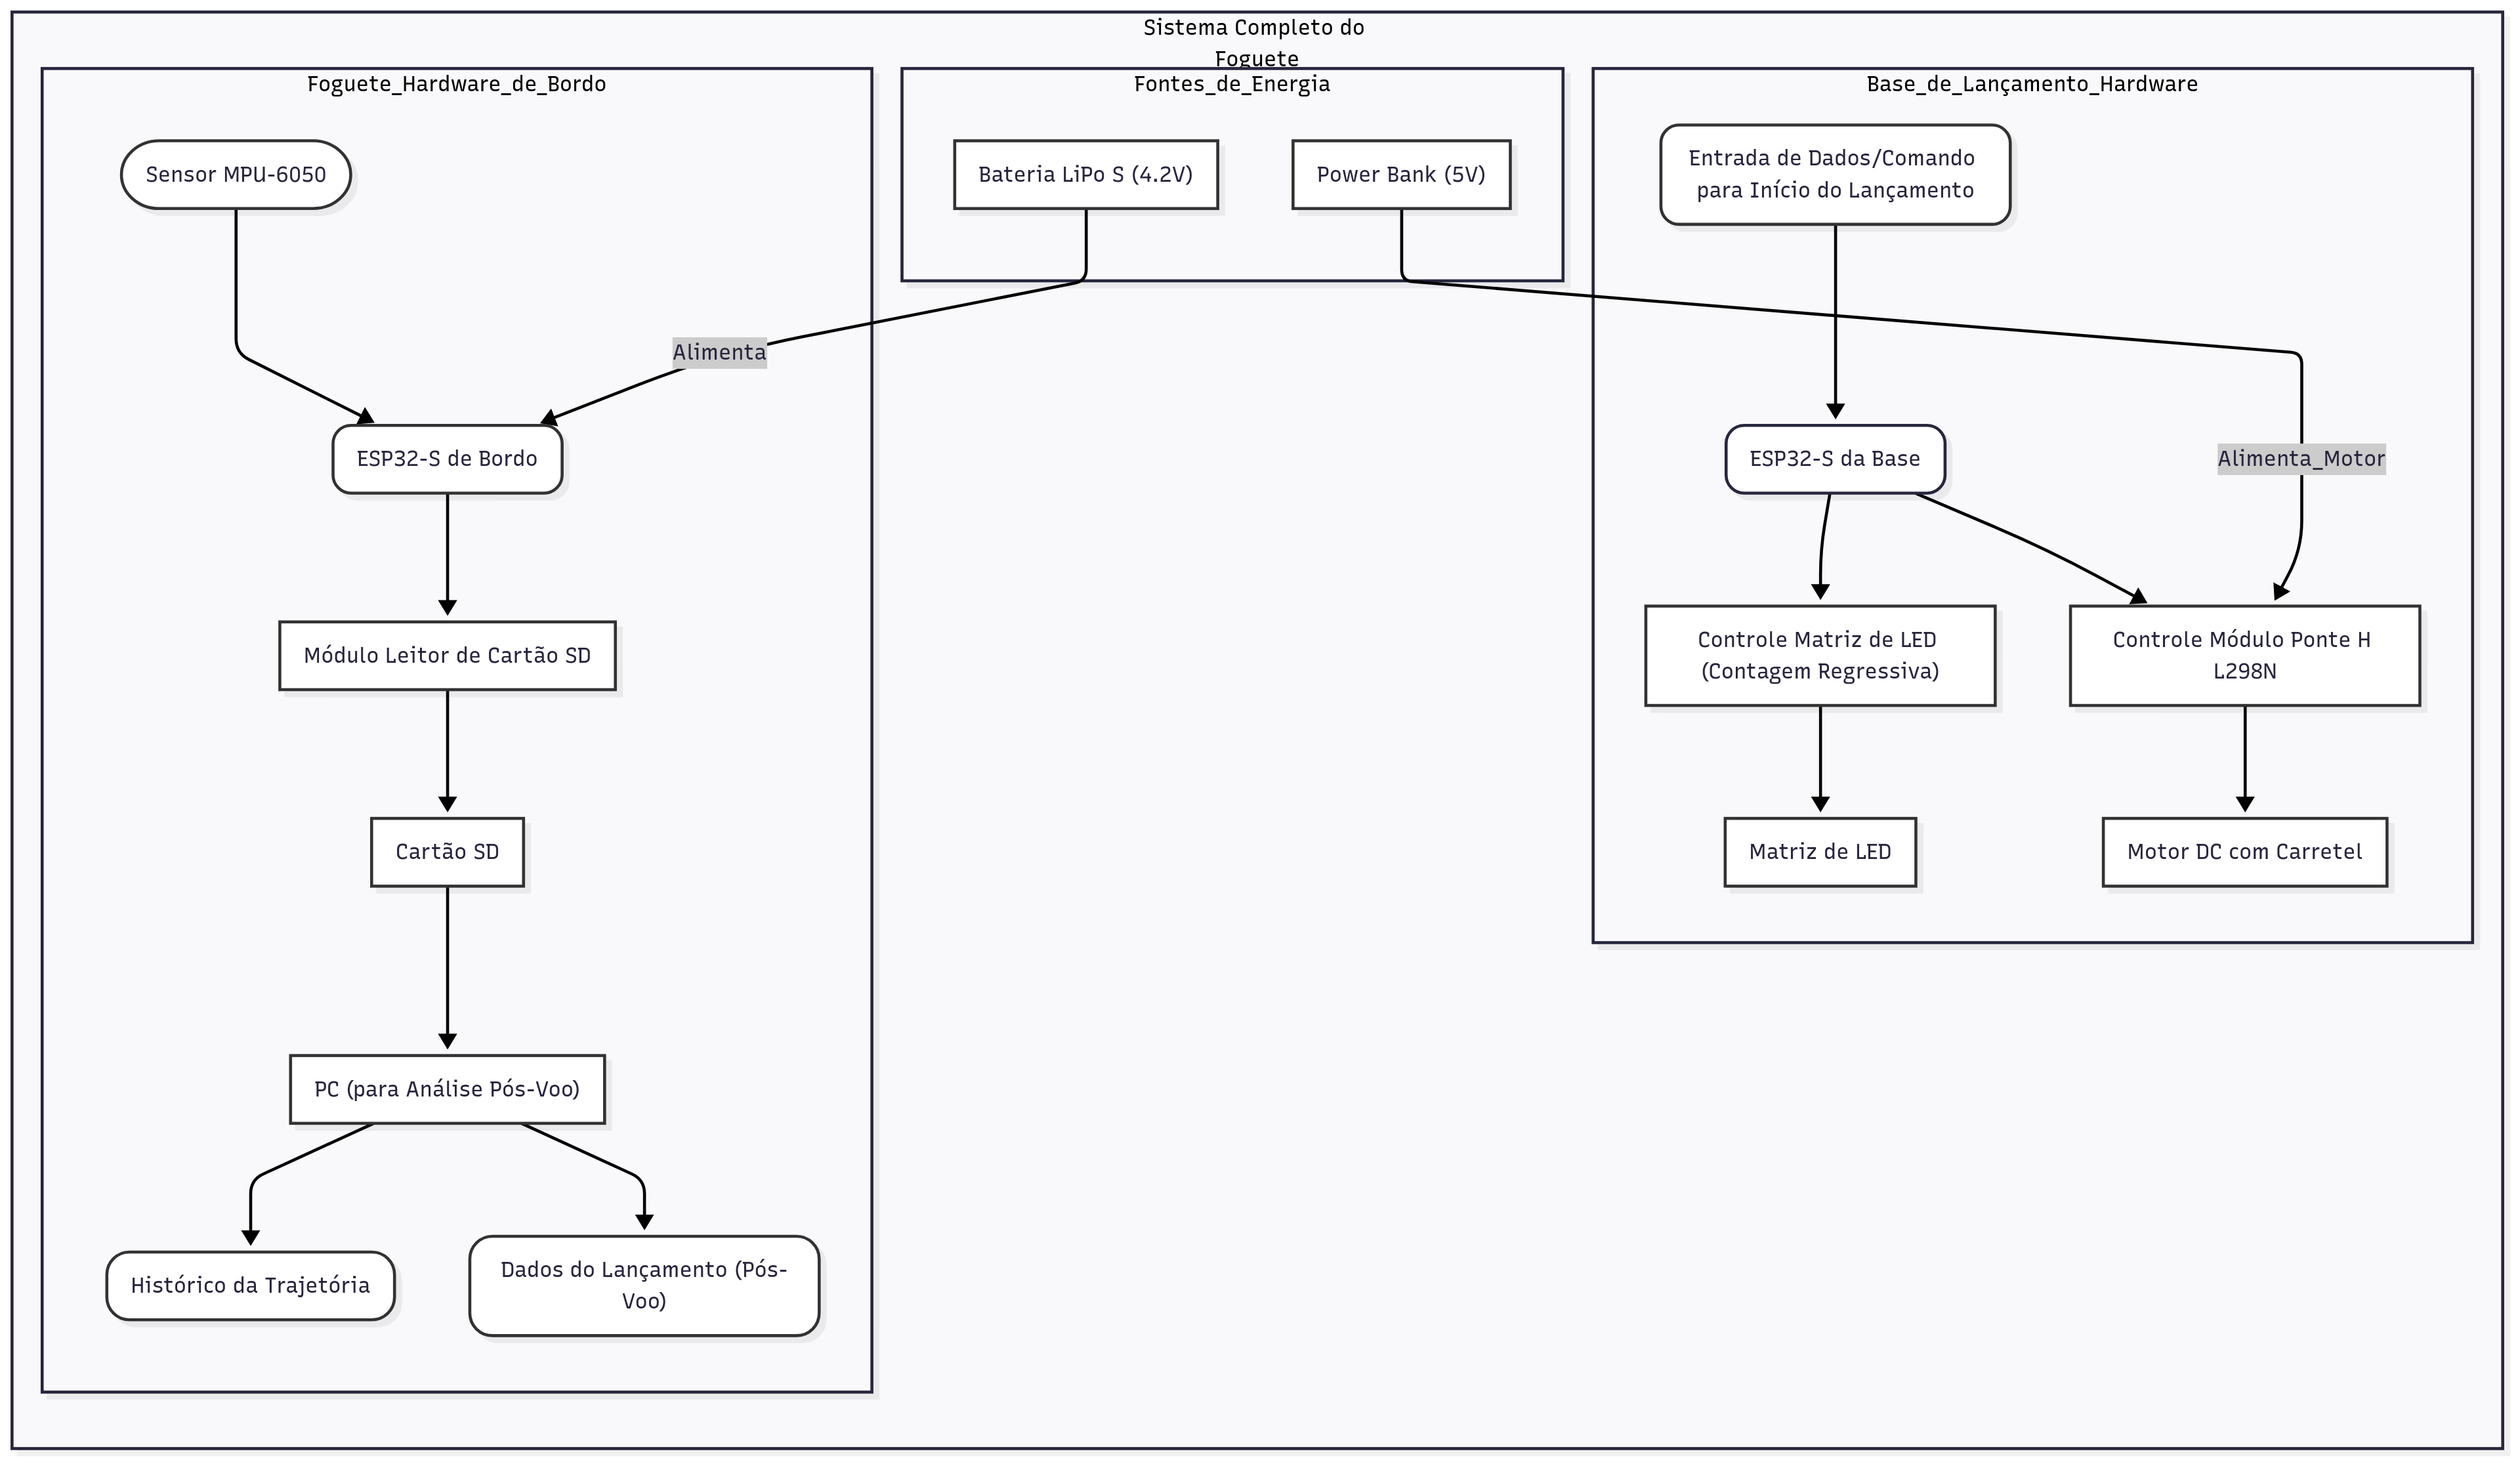
\includegraphics[width=\linewidth]{figuras/hardware/diagramaDeBlocos.png}
    \caption{Diagrama de Blocos de Hardware do Sistema Completo do Foguete}
    \label{fig:diagrama_blocos_embarcado}
\end{figure}

\subsection{Detalhes das Conexões e Pinos}
O diagrama de blocos acima ilustra a interconexão dos componentes de hardware do foguete d'água. Abaixo, encontra-se as conexões e pinos utilizados para cada componente, tanto no subsistema a bordo do foguete quanto no subsistema da base de lançamento.

\subsubsection{Conexões da ESP32 (Base do Foguete)}

\begin{itemize}
    \item Bateria Positivo (+) $\rightarrow$ ESP32 Vin: A entrada Vin do ESP32 aceita tensões mais altas e possui um regulador interno para fornecer a tensão de operação de 3.3V. 
    \item Bateria Negativo (-) $\rightarrow$ ESP32 GND: Todos os dispositivos compartilharão um terra comum para garantir o correto funcionamento do circuito.
    \item Um cabo USB do Power Bank (5V) será conectado à entrada MicroUSB do ESP32 da base para alimentá-lo. 
    \item Um segundo cabo USB, com suas extremidades cortadas, terá seus fios positivo e negativo conectados diretamente às entradas de alimentação correspondentes no módulo Ponte H L298N (positivo para a entrada de força do motor, e negativo para o GND da Ponte H), fornecendo os 5V necessários para energizar o motor DC.
\end{itemize}

\subsubsection{Conexões do MPU-6050}

\begin{itemize}
    \item O MPU-6050 utiliza o protocolo de comunicação I2C.
    \item ESP32 GPIO21 (SDA) $\rightarrow$ MPU-6050 SDA pin: O pino SDA (Serial Data) é utilizado para a transferência de dados seriais.
    \item ESP32 GPIO22 (SCL) $\rightarrow$ MPU-6050 SCL pin: O pino SCL (Serial Clock) é utilizado para a sincronização da transferência de dados.
    \item ESP32 3.3V pin $\rightarrow$ MPU-6050 VCC pin: O pino VCC fornece a alimentação de 3.3V necessária para o funcionamento do sensor.
    \item ESP32 GND pin $\rightarrow$ MPU-6050 GND pin: O pino GND fornece o terra para o sensor.
    \item MPU-6050 ADO pin $\rightarrow$ GND: O pino ADO é conectado ao terra para configurar o endereço I2C do MPU-6050 para $0\times68$.
\end{itemize}

\subsubsection{Conexões do Módulo de Cartão SD (MH-SD Card Module)}

\begin{itemize}
    \item O módulo de cartão SD utiliza o protocolo de comunicação SPI.
    \item ESP32 GPIO23 (MOSI) $\rightarrow$ MH-SD Card Module MOSI pin: O pino MOSI (Master Out Slave In) é utilizado para o ESP32 enviar dados para o cartão SD.
    \item ESP32 GPIO19 (MISO) $\rightarrow$ MH-SD Card Module MISO pin: O pino MISO (Master In Slave Out) é utilizado para o cartão SD enviar dados para o ESP32.
    \item ESP32 GPIO18 (SCK) $\rightarrow$ MH-SD Card Module SCK pin: O pino SCK (Serial Clock) é utilizado para a sincronização da transferência de dados.
    \item ESP32 GPIO5 (CS) $\rightarrow$ MH-SD Card Module CS pin (Chip Select): O pino CS é utilizado para selecionar o módulo de cartão SD. Este pino pode variar dependendo do módulo utilizado.
    \item ESP32 3.3V pin $\rightarrow$ MH-SD Card Module VCC pin: O pino VCC fornece a alimentação de 3.3V necessária para o funcionamento do módulo.
    \item ESP32 GND pin $\rightarrow$ MH-SD Card Module GND pin: O pino GND fornece o terra para o módulo.
\end{itemize}

\subsubsection{Conexões do Botão}

\begin{itemize}
    \item ESP32 GPIO27 $\rightarrow$ Um pino do Botão.
    \item GND da ESP32 $\rightarrow$ O outro pino do Botão. (Este pino será configurado com pull-up interno no firmware do ESP32).
\end{itemize}

\subsubsection{Conexões do Subsistema da Base de Lançamento}

\begin{itemize}
    \item ESP32 GPIO (pinos de dados, ex: via SPI ou GPIOs dedicados) $\rightarrow$ Matriz de LED (pinos de controle).
    \item ESP32 3.3V pin $\rightarrow$ Matriz de LED VCC pin.
    \item ESP32 GND pin $\rightarrow$ Matriz de LED GND pin.
\end{itemize}

\subsubsection{Conexões do Motor DC e Módulo Ponte H L298N}

\begin{itemize}
    \item ESP32 GPIO (PWM) $\rightarrow$ Ponte H L298N Enable (EN) pin: Para controle de velocidade.
    \item ESP32 GPIO (HIGH/LOW) $\rightarrow$ Ponte H L298N Input (IN1, IN2) pins: Para controle de direção.
    \item Ponte H L298N Output (OUT1, OUT2) pins $\rightarrow$ Motor DC.
    \item Ponte H L298N GND pin $\rightarrow$ GND da ESP32 da base (para terra comum).
    \item Ponte H L298N entrada de alimentação do motor (Vs/sense\_a) $\leftarrow$ Cabo USB cortado Positivo (do Power Bank).
\end{itemize}

% \newpage

\subsection{Esquemático de Circuito do Hardware de Bordo}
\begin{figure}[H]
    \centering
    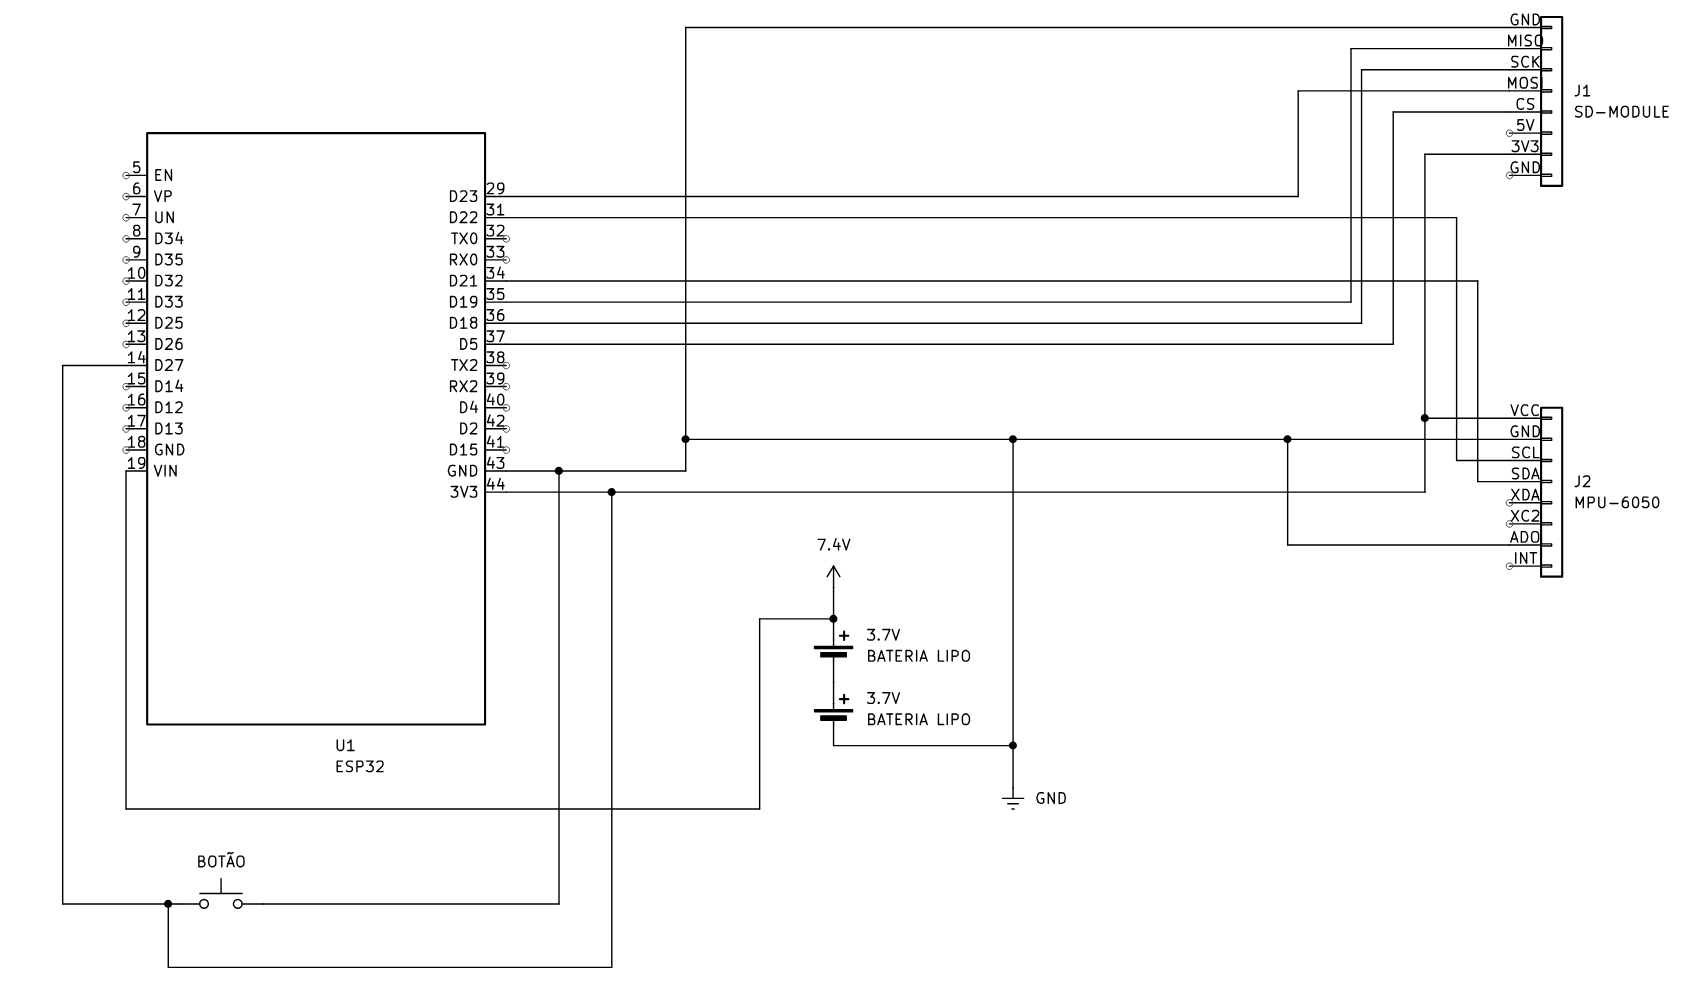
\includegraphics[width=\linewidth]{figuras/hardware/esquematico.png}
    \caption{Esquemático de Circuito do Hardware de Bordo do Foguete}
    \label{fig:esquematico_de_bordo}
\end{figure}

% \newpage

\subsection{Esquemático de Circuito do Hardware da Base de Lançamento}

\begin{figure}[H]
    \centering
    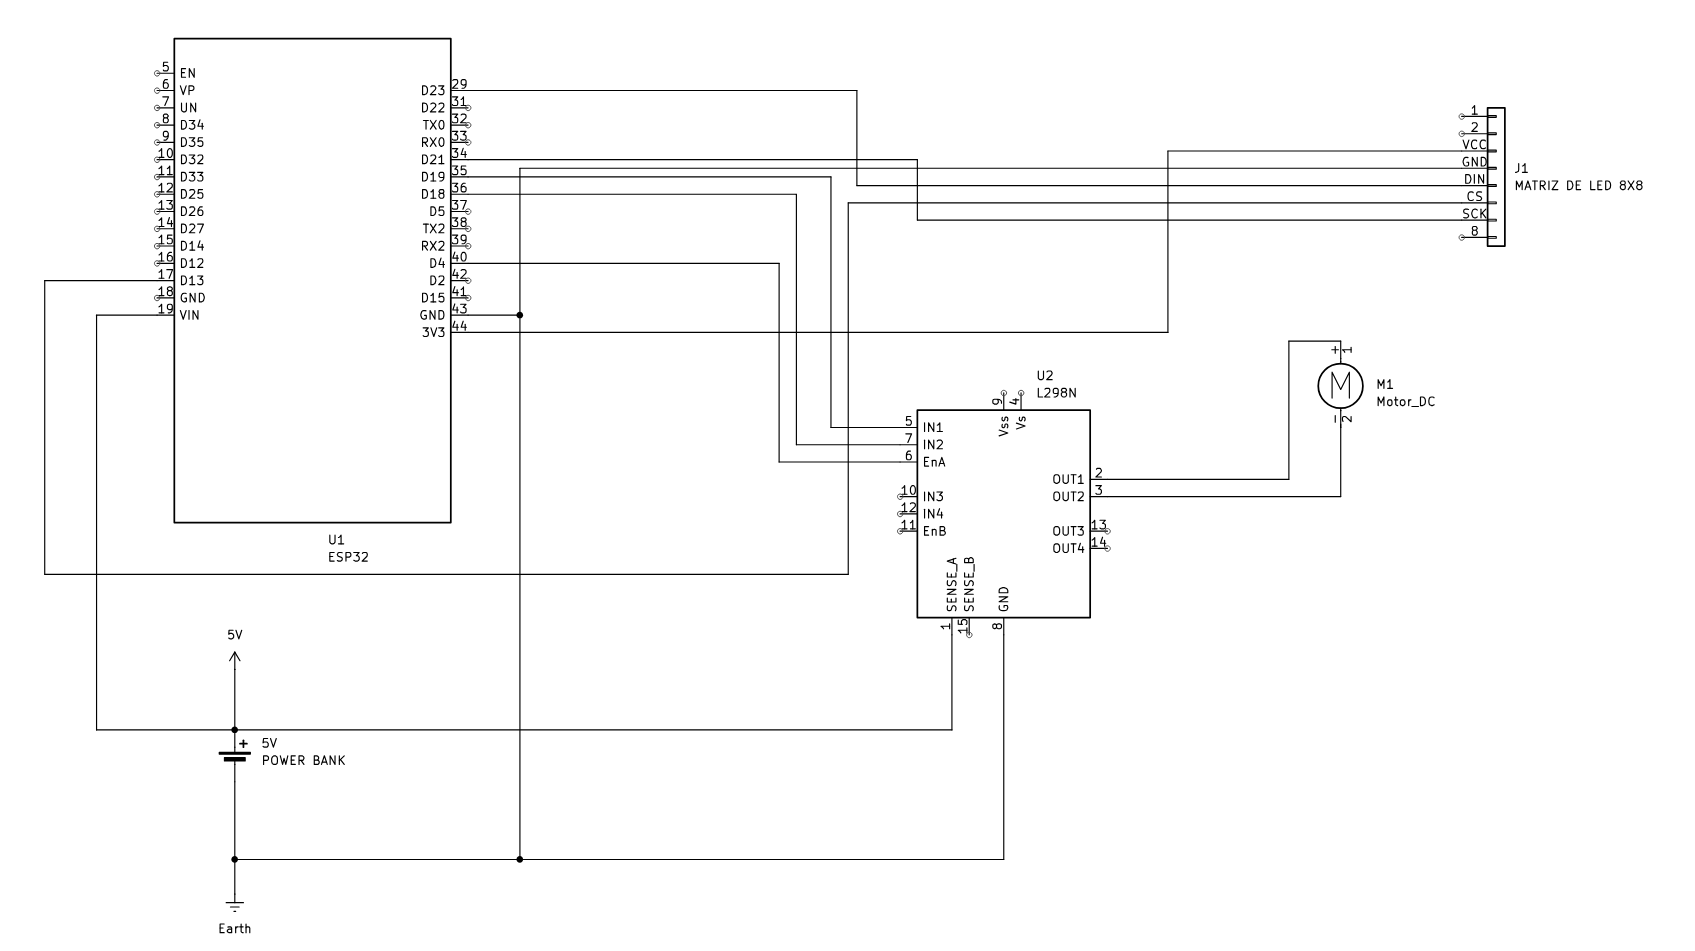
\includegraphics[width=\linewidth]{figuras/hardware/esquematicoBase.png}
    \caption{Esquemático de Circuito do Hardware da Base de Lançamento}
    \label{fig:esquematico_base}
\end{figure}

% \newpage

\subsection{Lançamento do Foguete}
O processo de lançamento do foguete é a  fase crítica que demanda precisão e controle sequencial por parte do sistema de hardware e firmware. Por isso, a automação deste processo é gerenciada pelo microcontrolador ESP32, que então coordena a contagem regressiva visual e o acionamento mecânico final.

A sequência de lançamento é iniciada por um comando ou evento detectado pelo ESP32. Embora o método exato de disparo possa ser configurado, uma vez acionado, o firmware executa as seguintes etapas controladas:

\begin{figure}[H]
    \centering
    \includegraphics[width=0.9\textwidth,height=1\textheight,keepaspectratio]{figuras/hardware/diagramaDeLançamento.png}
    \caption{Diagrama de Lançamento do Foguete}
    \label{fig:diagrama_lancamento}
\end{figure}

\begin{enumerate}
    \item Início da Contagem Regressiva: Após o comando de lançamento, o ESP32 ativa uma matriz de LEDs. Esta matriz serve como um indicador visual claro da contagem regressiva, exibindo os segundos restantes para o lançamento (e.g., de 9 a 1). Este feedback visual é essencial para a segurança e para a sincronização da equipe durante as operações de campo.
    \item Controle do Motor DC e Módulo Ponte H: Concomitantemente à contagem regressiva, ou imediatamente após sua conclusão, o ESP32 envia sinais de controle para o módulo Ponte H L298N. Este módulo, por sua vez, gerencia o motor DC (5V). A lógica de controle envolve um comando para o motor girar no sentido horário por dois segundos, seguido de uma pausa de dois segundos, e então um comando para o motor girar no sentido anti-horário. Esta sequência permite o acionamento preciso de um carretel acoplado ao eixo do motor.
    \item Acionamento Mecânico: No contexto do sistema de lançamento do foguete, o motor DC, através do carretel acoplado ao seu eixo, enrola ou desenrola uma linha que está conectada à trava do foguete. Ao receber o comando do ESP32 via Ponte H, o motor gira, puxando a linha e liberando a trava para o lançamento. A capacidade de girar em ambos os sentidos (horário e anti-horário) é essencial para que seja possível recolocar a trava do foguete após o lançamento ou para testes.
\end{enumerate}


% \newpage

